\section{Introduction}

% ===== 第1段：业务问题（决策导向） =====
Forging is the primary forming process for load-bearing components in the aerospace, energy, and automotive sectors, where forming quality governs in-service safety and production efficiency and cost determine enterprise profitability. Forging production must therefore minimize forming time and maximize throughput while guaranteeing quality. As shown in Fig.~\ref{fig:forging_press}, the workpiece undergoes plastic deformation under compression between the upper and lower dies, and the die speed is the downward velocity of the upper die. This speed profile affects the thermo-mechanical response and dynamic softening of the material through its control of the strain rate~\cite{lin2011critical}, and simultaneously determines forging time and workpiece damage, thereby influencing throughput and quality~\cite{bambach2018towards}. How to set the die speed profile is thus the core decision problem for efficient, high-quality forging.

\begin{figure}[htbp]
\centerline{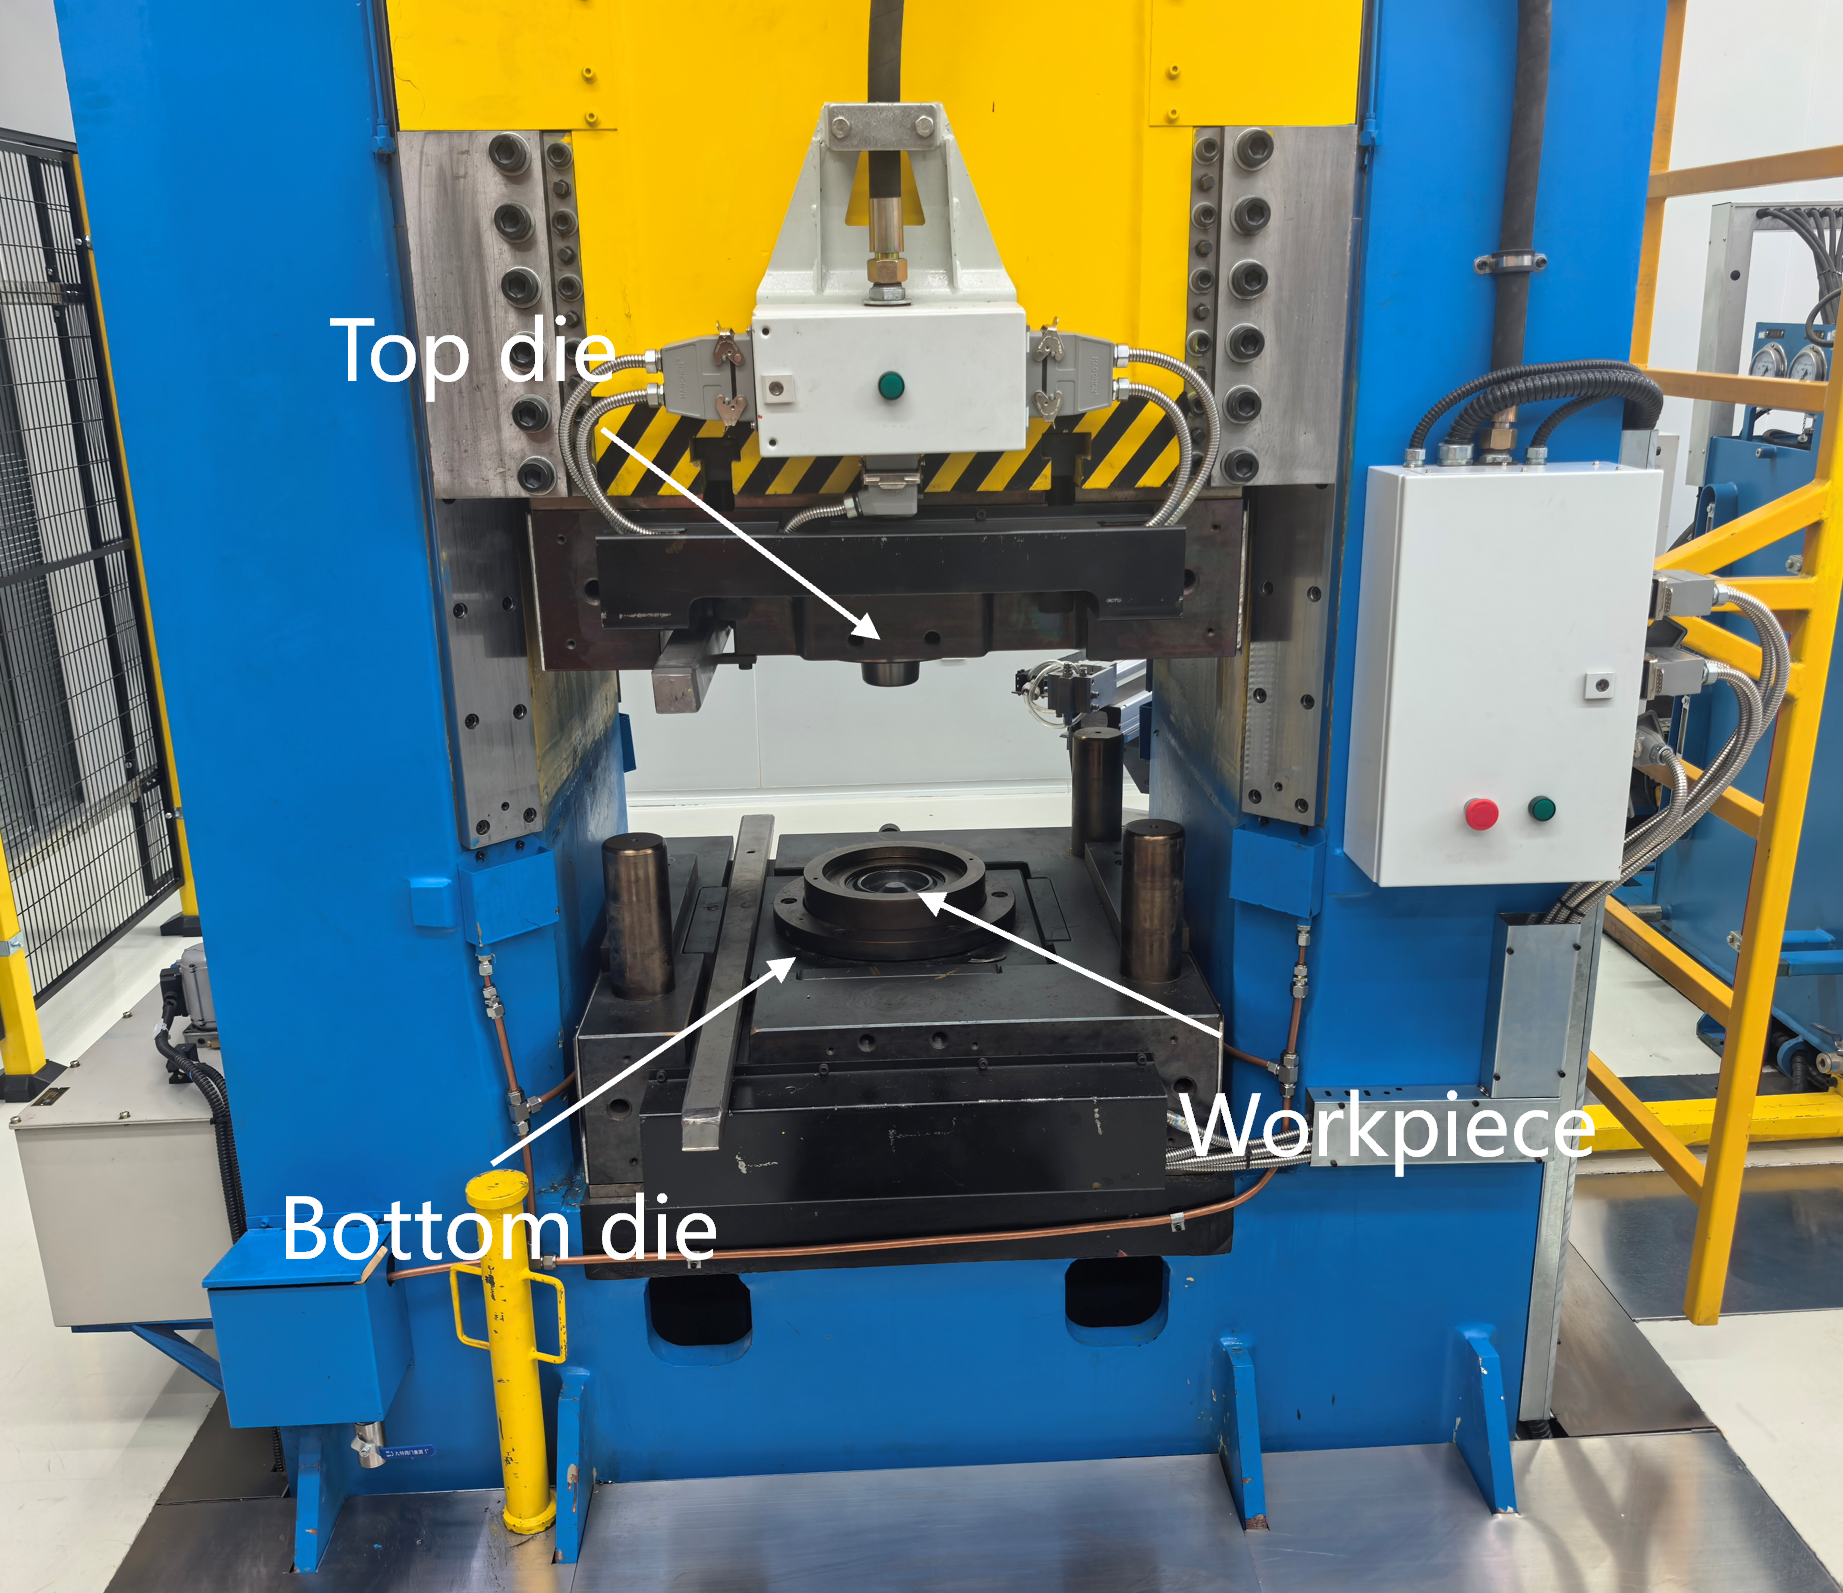
\includegraphics[width=7cm]{forging_press.png}}
\caption{Schematic of the forging press.}
\label{fig:forging_press}
\end{figure}

% ===== 第2段：研究意义（决策导向） =====
This work aims to intelligently determine the die speed profile under varying initial workpiece temperatures. Before forging, workpieces are preheated to different temperatures in a furnace; owing to transfer delays and differential heat loss between extraction and clamping, the initial temperature of each batch fluctuates, which in turn affects the deformation resistance and damage evolution throughout the process. Since the die speed can vary continuously over the entire forging history, the speed profile can flexibly modulate the pressing rate along with the evolution of temperature and deformation, minimizing forging time while keeping the workpiece free of cracking, and thereby raising throughput, lowering cost, and reducing equipment and die wear. Compared with constant-speed or low-dimensional piecewise schemes, a continuous speed profile offers higher degrees of freedom and process adaptability, exploiting the dynamic softening of the material more fully.

% ===== 第3段：已有工作①锻造工艺智能决策 =====
Existing work on intelligent decision-making for forging process parameters falls into three categories. Metaheuristic algorithms such as particle swarm optimization and NSGA-II search the parameter space with a finite-element or material model as the objective~\cite{chen2019strategy, ding2024enhancing}; however, each fitness evaluation requires a full simulation, and the optimized variables are mostly scalar parameters that cannot represent a speed profile varying continuously along the deformation history. Surrogate models instead fit a machine-learning mapping from process parameters to outcomes, such as predicting the strain distribution along the axis of a single pass~\cite{dischino2021open} or replacing finite elements with a graph neural network to predict the final-state field~\cite{shivaditya2022graph}; yet their outputs correspond to a single forming operation or one final state, lacking evolution along time steps and thus unable to provide the process state needed for stepwise decision-making. Control-based methods directly learn process policies, e.g., designing passes with deep Q-learning~\cite{reinisch2021successful}, and online adjustment of rolling speed~\cite{zhang2020online}, heating~\cite{ma2022using}, and TNM-B1 forging control~\cite{stendal2024developing}; but their actions are mostly discrete or low-dimensional setpoints and rely on online feedback, so they cannot provide a stepwise-adjustable continuous speed profile under offline conditions.

% ===== 第4段：已有工作②决策与控制方法 =====
A single forging operation is short, the internal stress and damage fields of the workpiece cannot be measured in real time, the temperature field can only be captured at the surface, and the system response latency is large; online closed-loop control based on real-time sensor feedback is thus impractical, and the speed profile can only be determined offline before production. Model predictive control requires online receding-horizon optimization and relies on real-time state feedback~\cite{kouvaritakis2016model}, but the internal state is unobservable and the latency is large, making receding-horizon optimization hard to implement. Iterative learning control depends on the repeatability of operating conditions~\cite{ahn2007iterative}, yet the temperature and clamping conditions of forging fluctuate batch by batch, so the repeatability assumption rarely holds. Online reinforcement learning requires repeated interaction with the environment~\cite{dharmadhikari2023reinforcement}, but forging experiments are costly and risky, making online exploration impractical. Offline reinforcement learning instead learns a policy from historical data~\cite{levine2020offline} and has been validated in process-industry scenarios such as hot rolling and thickeners~\cite{zhan2022deepthermal, 10705802}; however, its observations are mostly low-dimensional sensor readings and its actions are scalar setpoints, so it cannot accommodate point-cloud observations and function-level actions. World-model methods first learn environment dynamics in a latent space and then train or plan a policy within the model~\cite{hafner2020mastering}, but their constraints are typically formulated as cumulative costs and their execution is online closed-loop feedback, which is inconsistent with the requirements of the stepwise damage constraints and the one-shot offline deployment of this work.

% ===== 第5段：已有工作③点云表征 =====
The observation required for forging decision-making is a point cloud that carries geometry together with temperature, von Mises stress, and damage at every step. Point-cloud deep models, exemplified by PointNet++, extract permutation-invariant features through hierarchical sampling and local aggregation~\cite{qi2017pointnetpp}; however, these models target classification and segmentation of static scenes and output class or segmentation labels rather than physical fields. Point-cloud generation models such as PCN, FoldingNet, and PointFlow reconstruct or generate point clouds from a latent variable~\cite{yuan2018pcn, yang2018foldingnet, li2019pointflow}; yet their reconstruction target is a static point cloud, so they neither capture the time-varying evolution of the point cloud driven by process conditions nor predict the geometry and fields at the next moment from a latent state.

% ===== 第6段：已有工作④连续时间演化建模 =====
Forging thermo-mechanical deformation evolves continuously in time. The finite element method is highly accurate but requires numerically solving the entire deformation history, taking hours to days per run~\cite{halici2014modelling}; any change in process parameters necessitates a full recomputation, so the cost cannot be amortized. End-to-end data-driven models provide only a single input-to-output mapping and therefore lack multi-step temporal prediction capability. Sequential models such as RNNs, LSTMs, and Transformers recur over discrete time steps~\cite{elman1990finding, hochreiter1997long, vaswani2017attention}; however, discrete step sizes do not correspond to the continuous loading of forging, making it difficult to capture the continuous physical evolution. Neural ODEs describe the continuous change of state via a vector field, offering a framework for continuous-time modeling, yet their application to high-dimensional point-cloud multi-physics prediction remains limited. The temperature, stress, and damage of forging are fields defined over a continuous geometry that evolve along the deformation history and must be queried at arbitrary locations; existing data-driven models mostly discretize fields onto a fixed grid or a fixed number of points, making it difficult to predict the entire field on continuous coordinates. Operator-learning models such as DeepONet model a field as a continuous function of coordinates and learn function-to-function mappings: the branch encodes the function input, the trunk queries with the coordinate as the independent variable, and all points share a spatial basis, so that a single network outputs field values at arbitrary coordinates---matching the need to reconstruct a continuous geometry--multi-physics field from a low-dimensional latent state.

% ===== 第7段：本文思路 =====
To address the above limitations, this work constructs a forging world model that takes an arbitrary continuous-time speed profile as input and jointly carries the evolution of geometry and multi-physics fields in a low-dimensional latent state, characterizing the forging thermo-mechanical process in continuous time while guaranteeing reconstruction and multi-step prediction accuracy, serving as a surrogate environment for decision training and inference. Building on this model, a continuous speed-profile policy is trained from offline data to output a smooth, continuous, and directly executable speed profile that satisfies the damage constraint, thereby realizing intelligent decision-making of the die speed profile.

% ===== 第8段：研究方法 =====
This work adopts a two-stage method, with the overall framework shown in Fig.~\ref{fig:framework}.

\textbf{Stage 1: world model training.}
We adopt an Encoder--Latent Dynamics--Decoder architecture: a hierarchical PointNet++ encoder compresses the point cloud of each step into a low-dimensional latent state that jointly carries geometry and multi-physics information; a Neural ODE with the speed profile as a physical prior models the continuous-time dynamics in the latent space; and a decoder performs residual reconstruction with the first-step geometry as the displacement base and regresses the physical fields from the first-step coordinates, realizing reconstruction and prediction of the point cloud.

\textbf{Stage 2: policy training.}
With the trained world model as the environment, the speed-profile decision is formulated as a finite-horizon constrained Markov decision process with safety constraints; the policy takes the world model's latent state as input and determines the die speed step by step along the deformation history, generating a smooth, continuous speed profile; the policy is trained via offline safe reinforcement learning, with the damage constraint handled by Lagrangian relaxation. At solving time, the world model performs stepwise decision-making: at each step the current speed is output conditioned on the world model's latent state, so that the entire profile adapts to the process state without relying on physical sensors; after solving, the resulting complete speed profile is deployed to the equipment once.

\begin{figure}[htbp]
\centerline{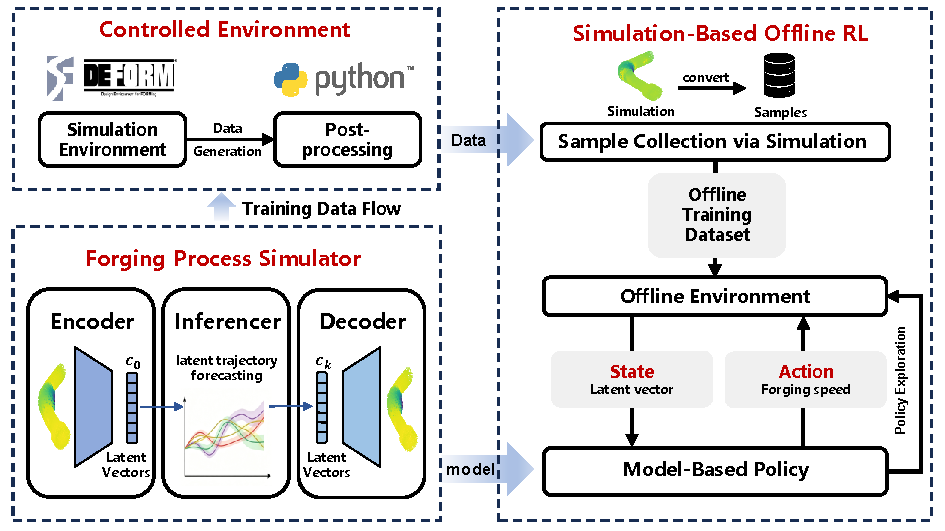
\includegraphics[width=12cm]{fram-1-wide.pdf}}
\caption{Overall framework of this work.}
\label{fig:framework}
\end{figure}

% ===== 第9段：研究贡献 =====
The main contributions are as follows:
\begin{enumerate}\setlength{\itemsep}{0pt}\setlength{\parsep}{0pt}
    \item \textbf{A forging world model for forging point-cloud sequences.}
    It jointly carries geometry and multi-physics fields in a low-dimensional latent state and models the controlled evolution process in continuous time via a Neural ODE, realizing reconstruction and multi-step prediction of the time-varying point-cloud process, and providing an efficient surrogate environment for decision training and inference.
    \item \textbf{Safe decision-making of continuous speed profiles based on the world model.}
    It solves offline within the world model to generate a smooth, continuous speed profile satisfying the damage constraint, which is then deployed to the equipment once, overcoming the representational limitations of conventional low-dimensional parameterization.
    \item \textbf{Practical validation.}
    The proposed method is applied to the forging of a 6082 aluminum alloy control arm, validating the prediction accuracy of the world model and the effectiveness of the decision scheme in the DEFORM simulation environment.
\end{enumerate}
